\chapter{并行结构的FIR滤波器设计}
\begin{introduction}
  \item \textit{乘法器IP核配置;}
  \item \textit{Verilog编写全并行结构FIR滤波器;}
  \item \textit{基于全并行结构的FIR滤波器FPGA实现。}
\end{introduction}
\section{实验背景与目的}
在现代数字信号处理(DSP)领域,FIR滤波器被广泛应用于信号的平滑、去噪、频率选择等任务。FIR滤波器的实现方式多种多样,基于FPGA(现场可编程门阵列)的实现因其并行处理能力和高效的硬件资源利用而成为常见的选择。本实验旨在通过基于FPGA的并行结构设计一个FIR滤波器,研究其实现过程并分析其资源消耗和时序性能。实验的主要目标是:
\begin{itemize}
    \item 设计并实现一个基于FPGA的并行结构FIR滤波器;
    \item 通过使用乘法器IP核优化滤波器的计算性能;
    \item 完成滤波器的FPGA实现,并进行资源消耗与时序性能的分析;
    \item 探讨如何提高该FIR滤波器的工作频率。
\end{itemize}

\section{实验原理}


\subsection{全并行结构FIR滤波器的实现}

在数字信号处理中,FIR滤波器是一种常用的线性时不变系统,能够有效地对输入信号进行滤波操作。为了提高处理速度并适应高速信号处理的需求,采用全并行结构实现FIR滤波器是一个有效的方式。在FPGA中实现全并行结构的FIR滤波器,主要包括以下几个部分:

\begin{enumerate}
    \item \textbf{输入数据存储}:输入信号 \( X[n] \) 被存储在一组移位寄存器中,这些寄存器按照时序顺序依次存储输入信号的历史样本数据。这些寄存器构成了滤波器的延迟单元。
    
    \item \textbf{加法器}:对于对称的滤波器系数,通过对称加法器对输入信号的不同延迟版本进行加和。这一操作减少了乘法器的使用,提高了设计效率。在实现中,通过多级加法器对输入信号进行并行加法处理。
    
    \item \textbf{乘法器}:每个加和后的输入信号与相应的滤波器系数 \( h[k] \) 进行乘法运算。为提高性能,设计中通常使用专用硬件乘法器,这些乘法器执行并行计算,处理每个延迟输入信号与滤波器系数的乘积。
    
    \item \textbf{加法汇总}:所有乘法结果通过加法器进行汇总,最终生成滤波器的输出。为了提高吞吐量,通常使用多级流水线加法器对乘法结果进行累加。
    
    \item \textbf{输出}:通过加法器的最终结果,获得滤波后的信号 \( Y[n] \),作为系统的输出。
\end{enumerate}

通过上述模块的并行实现,FIR滤波器能够在每个时钟周期内并行处理多个信号样本,从而大大提高了处理速度和效率。由于设计的FIR滤波器满足线性相位特性,因此可以省去一半的乘法器,进一步优化了硬件资源的利用。

\subsection{FPGA的主要资源}

FPGA(现场可编程门阵列)是一种灵活且高效的硬件平台,适用于多种数字电路设计。FPGA的主要资源包括:

\begin{enumerate}
    \item \textbf{查找表(LUTs,Look-Up Tables)}:用于实现基本的逻辑运算。LUT是FPGA的核心逻辑单元,通过查表的方式实现逻辑函数。复杂的逻辑操作会消耗更多的LUT资源。
    
    \item \textbf{寄存器(Registers)}:用于存储信号的状态,广泛应用于时序逻辑设计。每个寄存器通常需要一个时钟周期来更新其状态。
    
    \item \textbf{乘法器(Multipliers)}:硬件乘法器用于加速乘法运算。由于乘法是计算中最复杂的操作之一,FPGA提供专用的硬件乘法器以提高效率。
    
    \item \textbf{块RAM(Block RAM,BRAM)}:用于存储数据的内存资源,FPGA中提供多个BRAM块,可用于存储大量数据,如滤波器的中间计算结果。
    
    \item \textbf{时钟资源}:FPGA内部包含多个时钟源,用于驱动不同的时钟域。时钟设计在FPGA中非常重要,合理的时钟管理可以优化系统性能。
    
    \item \textbf{输入输出引脚(I/O Pins)}:FPGA通过I/O引脚与外部世界进行数据交换,设计中的I/O需求会消耗一定的资源。
    
    \item \textbf{逻辑块(Logic Blocks)}:每个FPGA包含多个逻辑块,通常由多个LUT、寄存器和其他功能单元组成。设计时的逻辑块使用量直接影响FPGA的资源消耗。
\end{enumerate}

\subsection{时序与资源分析的重要性}

时序和资源分析是FPGA设计过程中不可或缺的一部分,其重要性体现在以下几个方面:

\begin{enumerate}
    \item \textbf{时序分析}:时序分析确保设计满足时钟约束,即确保设计中的信号在正确的时钟边缘触发,并且信号能够在规定的时间内稳定。时序问题可能导致信号错误传输,从而影响系统的正常运行。通过时序分析,可以识别设计中存在的潜在时序问题,如时序余量不足、时钟频率限制等问题,并采取措施进行优化。
    
    \item \textbf{资源分析}:FPGA的资源有限,设计中不同模块会消耗不同类型的资源(如LUT、寄存器、BRAM等)。资源消耗分析能够帮助设计者了解设计中哪些部分消耗了大量资源,从而采取优化措施。例如,可以通过减少不必要的逻辑单元、使用更高效的算法或者共享资源来减少FPGA资源的占用,降低功耗并提高系统性能。
    
    \item \textbf{优化设计}:通过时序和资源分析,设计者可以识别瓶颈,并采取相应的优化措施。例如,时序优化可能包括调整时钟频率、使用更高效的时钟分配方案;资源优化可能包括使用更紧凑的算法、共享硬件资源或将设计分割成多个模块,以便在不同的FPGA资源中均匀分配。
\end{enumerate}

综上所述,时序和资源分析不仅能够确保设计的正确性,还能帮助设计者有效地利用FPGA资源,最大化其性能并降低系统的成本。

\section{实验使用软件/平台}
\begin{itemize}
  \item Xilinx Vivado 2024.2;
  \item eNodeX 30B软件无线电创新平台;
  \item 示波器。
  \item MATLAB \& Simulink R2024b;
\end{itemize}
\section{实验内容}
\subsection{乘法器IP核配置}
在本例中,生成的FIR滤波器系数为12位有符号数,而待滤波数据经过对称相加后,需要支持13位有符号数。因此需要例化一个$13\times 12$的有符号数乘法器。由于不需要设计流水线,故对乘法器没有控制要求,因此取消同步控制信号和时钟Enable信号,降低设计复杂度。乘法器配置如图~\ref{fig:exp5:mult}。
\begin{figure}[htbp]
  \centering
  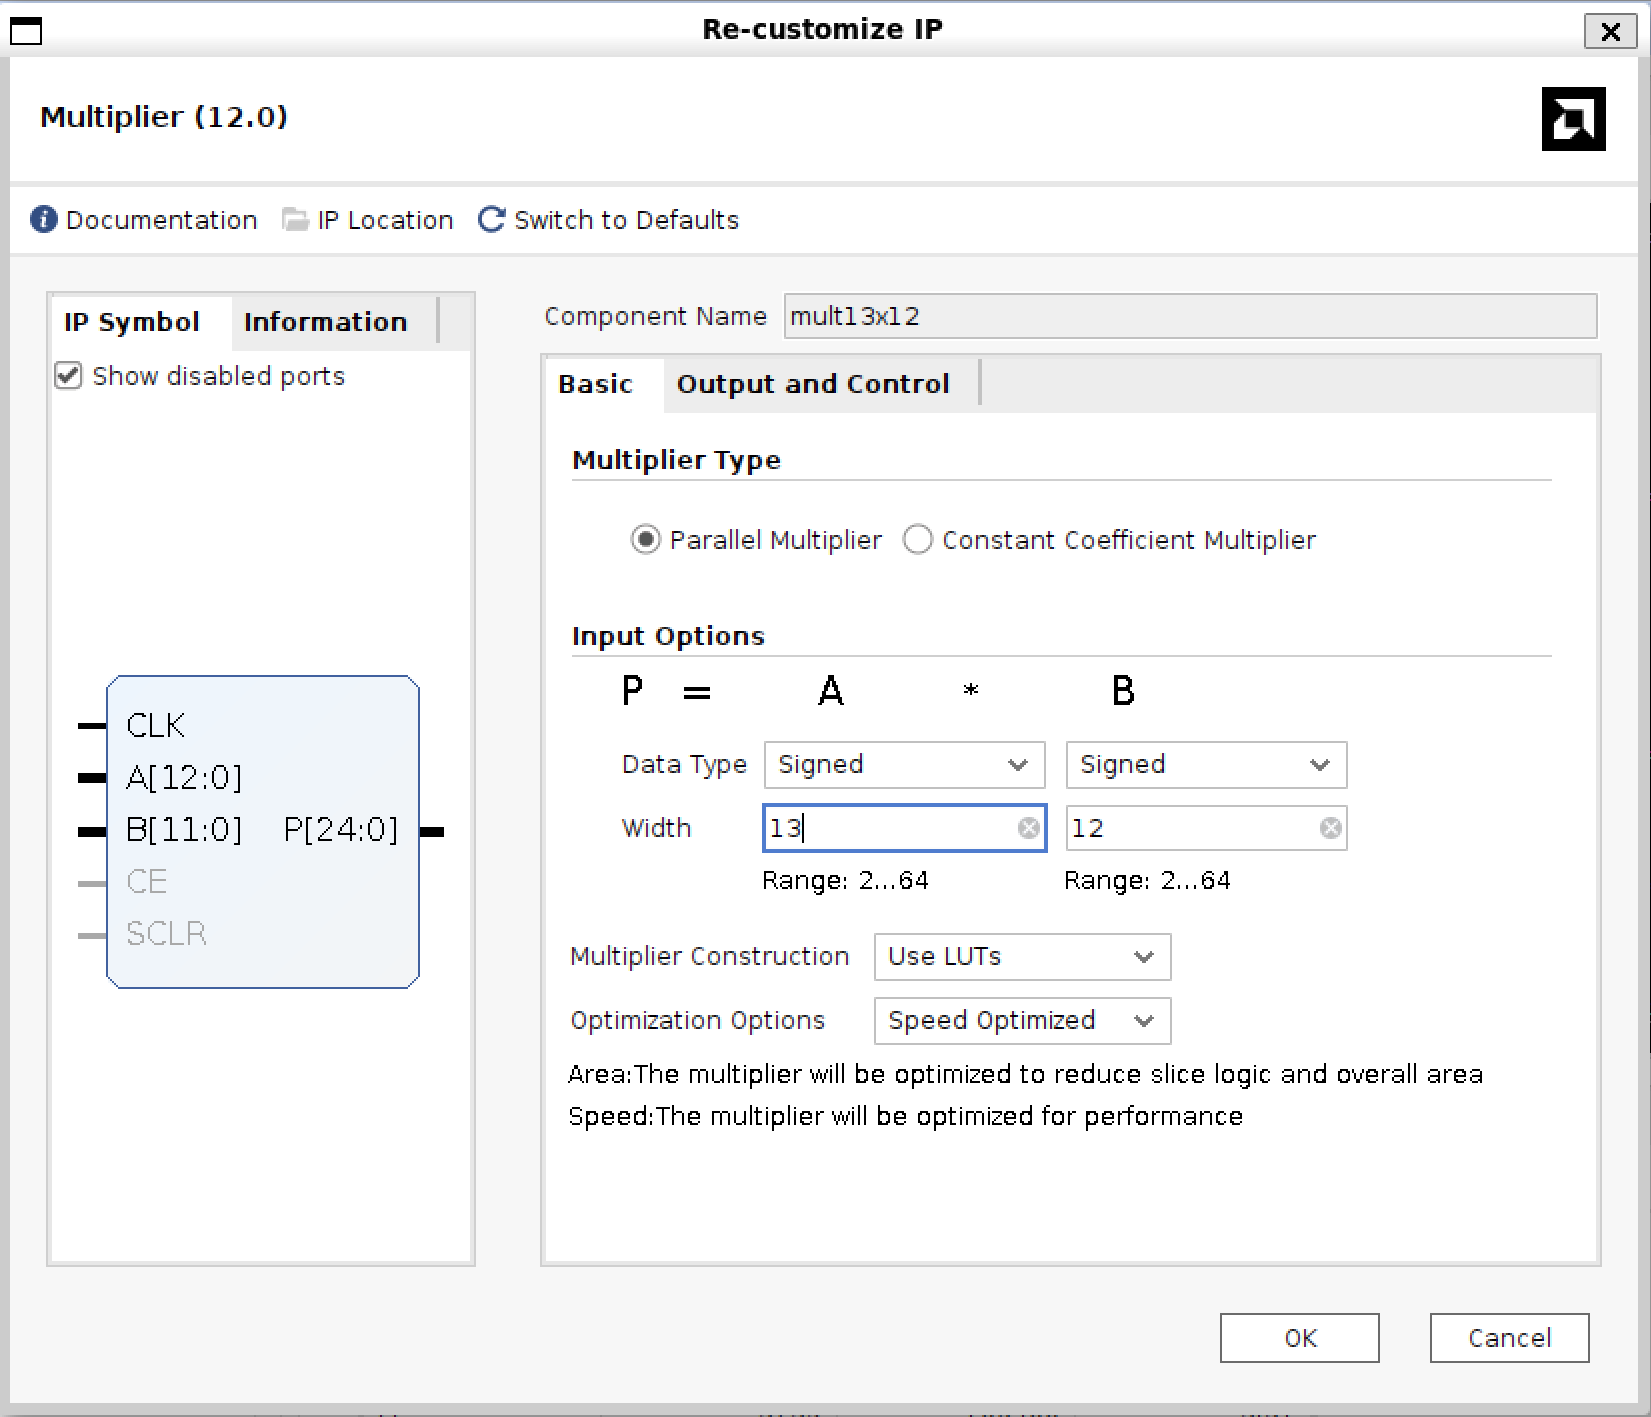
\includegraphics[width=0.75\textwidth]{figure/exp5/mult_settings.png}
  \caption{乘法器配置}
  \label{fig:exp5:mult}
\end{figure}

\subsection{全并行结构FIR滤波器的FPGA实现}
设计一个全并行的FIR滤波器,其输入输出端口如表~\ref{table:interface_fir_exp5}~所示。由于引入乘法器,输出信号位宽约为输入信号位宽的2倍。

\begin{table}[htbp]
  \centering
  \begin{tabular}{ccc}
    \toprule
     信号名 & 意义 & 端口类型\\
    \midrule
      \texttt{clk} & 50MHz时钟信号 & Input \\
     \texttt{Xin} & 12-bit 加和后量化正弦信号 & Input \\
     \texttt{Yout} & 26-bit 滤波后量化信号输出 & Output \\
    \bottomrule
  \end{tabular}
  \caption{FIR模块接口说明}
  \label{table:interface_fir_exp5}
\end{table}

下面的Verilog模块实现了一个全并行、全展开的FIR滤波器。输入信号 \texttt{Xin} 被存储在16个寄存器中,之后通过加法器对称相加。利用8个乘法器与MATLAB计算好的滤波器系数进行乘法运算,并通过两级流水线对结果进行加法汇总,最终输出滤波结果 \texttt{Yout}。

\begin{remark}
  \kaishu{由于该滤波器$N$为偶数且接近偶对称,故可以推断其为低通或带通滤波器,如设计好均可滤除8MHz的高频信号。}
\end{remark}
\begin{lstlisting}[language=verilog,caption={FIR滤波器模块}]
  `timescale 1ns / 1ps
  module fir_parallel( 
      input clk,            // 系统时钟
      input signed [11:0] Xin, // 输入数据
      output signed [25:0] Yout // 输出数据
  );
  
      // 定义滤波器系数
      parameter signed [11:0] coeff_b0 = -12'd116;
      parameter signed [11:0] coeff_b1 = -12'd111;
      parameter signed [11:0] coeff_b2 = -12'd22;
      parameter signed [11:0] coeff_b3 = 12'd243;
      parameter signed [11:0] coeff_b4 = 12'd692;
      parameter signed [11:0] coeff_b5 = 12'd1239;
      parameter signed [11:0] coeff_b6 = 12'd1743;
      parameter signed [11:0] coeff_b7 = 12'd2047;
  
      // 将数据存入移位寄存器Xin_Reg中
      reg signed [11:0] Xin_Reg[15:0];
      always @(posedge clk) begin
          Xin_Reg[0] <= Xin;
          Xin_Reg[1] <= Xin_Reg[0];
          Xin_Reg[2] <= Xin_Reg[1];
          Xin_Reg[3] <= Xin_Reg[2];
          Xin_Reg[4] <= Xin_Reg[3];
          Xin_Reg[5] <= Xin_Reg[4];
          Xin_Reg[6] <= Xin_Reg[5];
          Xin_Reg[7] <= Xin_Reg[6];
          Xin_Reg[8] <= Xin_Reg[7];
          Xin_Reg[9] <= Xin_Reg[8];
          Xin_Reg[10] <= Xin_Reg[9];
          Xin_Reg[11] <= Xin_Reg[10];
          Xin_Reg[12] <= Xin_Reg[11];
          Xin_Reg[13] <= Xin_Reg[12];
          Xin_Reg[14] <= Xin_Reg[13];
          Xin_Reg[15] <= Xin_Reg[14];
      end
  
      // 采用8个双输入加法器,完成对称系数相加
      // 两个12比特数据相加,需要用13比特数据存储数据
      reg signed [12:0] Xin_Add [7:0];
      always @(posedge clk) begin
          Xin_Add[0] = Xin_Reg[0] + Xin_Reg[15];
          Xin_Add[1] = Xin_Reg[1] + Xin_Reg[14];
          Xin_Add[2] = Xin_Reg[2] + Xin_Reg[13];
          Xin_Add[3] = Xin_Reg[3] + Xin_Reg[12];
          Xin_Add[4] = Xin_Reg[4] + Xin_Reg[11];
          Xin_Add[5] = Xin_Reg[5] + Xin_Reg[10];
          Xin_Add[6] = Xin_Reg[6] + Xin_Reg[9];
          Xin_Add[7] = Xin_Reg[7] + Xin_Reg[8];
      end
  
      // 实例化8个有符号数乘法器IP核mult,
      // 1级流水线延时输出
      wire signed [24:0] Mout [7:0];
      mult13x12 u0 (.CLK(clk), .A(Xin_Add[0]), .B(coeff_b0), .P(Mout[0]));
      mult13x12 u1 (.CLK(clk), .A(Xin_Add[1]), .B(coeff_b1), .P(Mout[1]));
      mult13x12 u2 (.CLK(clk), .A(Xin_Add[2]), .B(coeff_b2), .P(Mout[2]));
      mult13x12 u3 (.CLK(clk), .A(Xin_Add[3]), .B(coeff_b3), .P(Mout[3]));
      mult13x12 u4 (.CLK(clk), .A(Xin_Add[4]), .B(coeff_b4), .P(Mout[4]));
      mult13x12 u5 (.CLK(clk), .A(Xin_Add[5]), .B(coeff_b5), .P(Mout[5]));
      mult13x12 u6 (.CLK(clk), .A(Xin_Add[6]), .B(coeff_b6), .P(Mout[6]));
      mult13x12 u7 (.CLK(clk), .A(Xin_Add[7]), .B(coeff_b7), .P(Mout[7]));
  
      // 采用2级流水线完成8输入加法运算
      reg signed [26:0] sum1, sum2;
      reg signed [27:0] sum;
      always @(posedge clk) begin
          sum1 <= Mout[0] + Mout[1] + Mout[2] + Mout[3];
          sum2 <= Mout[4] + Mout[5] + Mout[6] + Mout[7];
          sum <= sum1 + sum2;
      end
  
      assign Yout = sum[25:0];
  
  endmodule
  \end{lstlisting}

基于此模块设计,编写测试模块(Testbench)如下。在测试模块中调用\textit{DDS Compiler} IP核生成1MHz和8MHz的正弦信号并相加后,对FIR模块进行测试。
\begin{lstlisting}[language=verilog, caption={Testbench文件}]
  `timescale 1ns / 1ps

module tb_FIR_PARALLEL;

    reg clk; // 时钟信号
    wire signed [11:0] xin; // FIR 输入信号
    wire signed [25:0] yout; // FIR 输出信号
    wire signed [11:0] sin1M, sin8M; // DDS 产生的两个输入信号

    fir_parallel sim (
        .clk(clk),
        .Xin(xin),  // 确保正确连接输入信号
        .Yout(yout) // 确保正确连接输出信号
    );

    // 产生 50MHz 的时钟信号
    initial begin
        clk = 0;
        forever #10 clk = ~clk;
    end

    // 实例化 SIN_1M 模块
    SIN_1M sin_1M (
        .aclk(clk),                                  // 输入时钟信号
        .s_axis_config_tvalid(1'b1),  // 配置有效信号
        .s_axis_config_tdata(16'H51E),    // 配置数据
        .m_axis_data_tvalid(),      // 数据有效信号
        .m_axis_data_tdata(sin1M)        // 输出数据
    );

    // 实例化 SIN_8M 模块
    SIN_8M sin_8M (
        .aclk(clk),                                  // 输入时钟信号
        .s_axis_config_tvalid(1'b1),  // 配置有效信号
        .s_axis_config_tdata(16'H28F5),    // 配置数据
        .m_axis_data_tvalid(),      // 数据有效信号
        .m_axis_data_tdata(sin8M)        // 输出数据
    );

    // 计算输入信号 xin
    assign xin = sin1M + sin8M;  // 将两个信号相加作为 FIR 输入信号

endmodule

  
\end{lstlisting}

测试结果如图~\ref{fig:exp5:result}~所示。\footnote{需要在xsim中调整数据格式(Radix)为Signed Decimal,波形格式为Analog。}可以看出设计的FIR滤波器成功滤除了高频的8MHz信号,而保留了1MHz的信号,这符合低通滤波器的特性。
\begin{figure}[htbp]
  \centering
  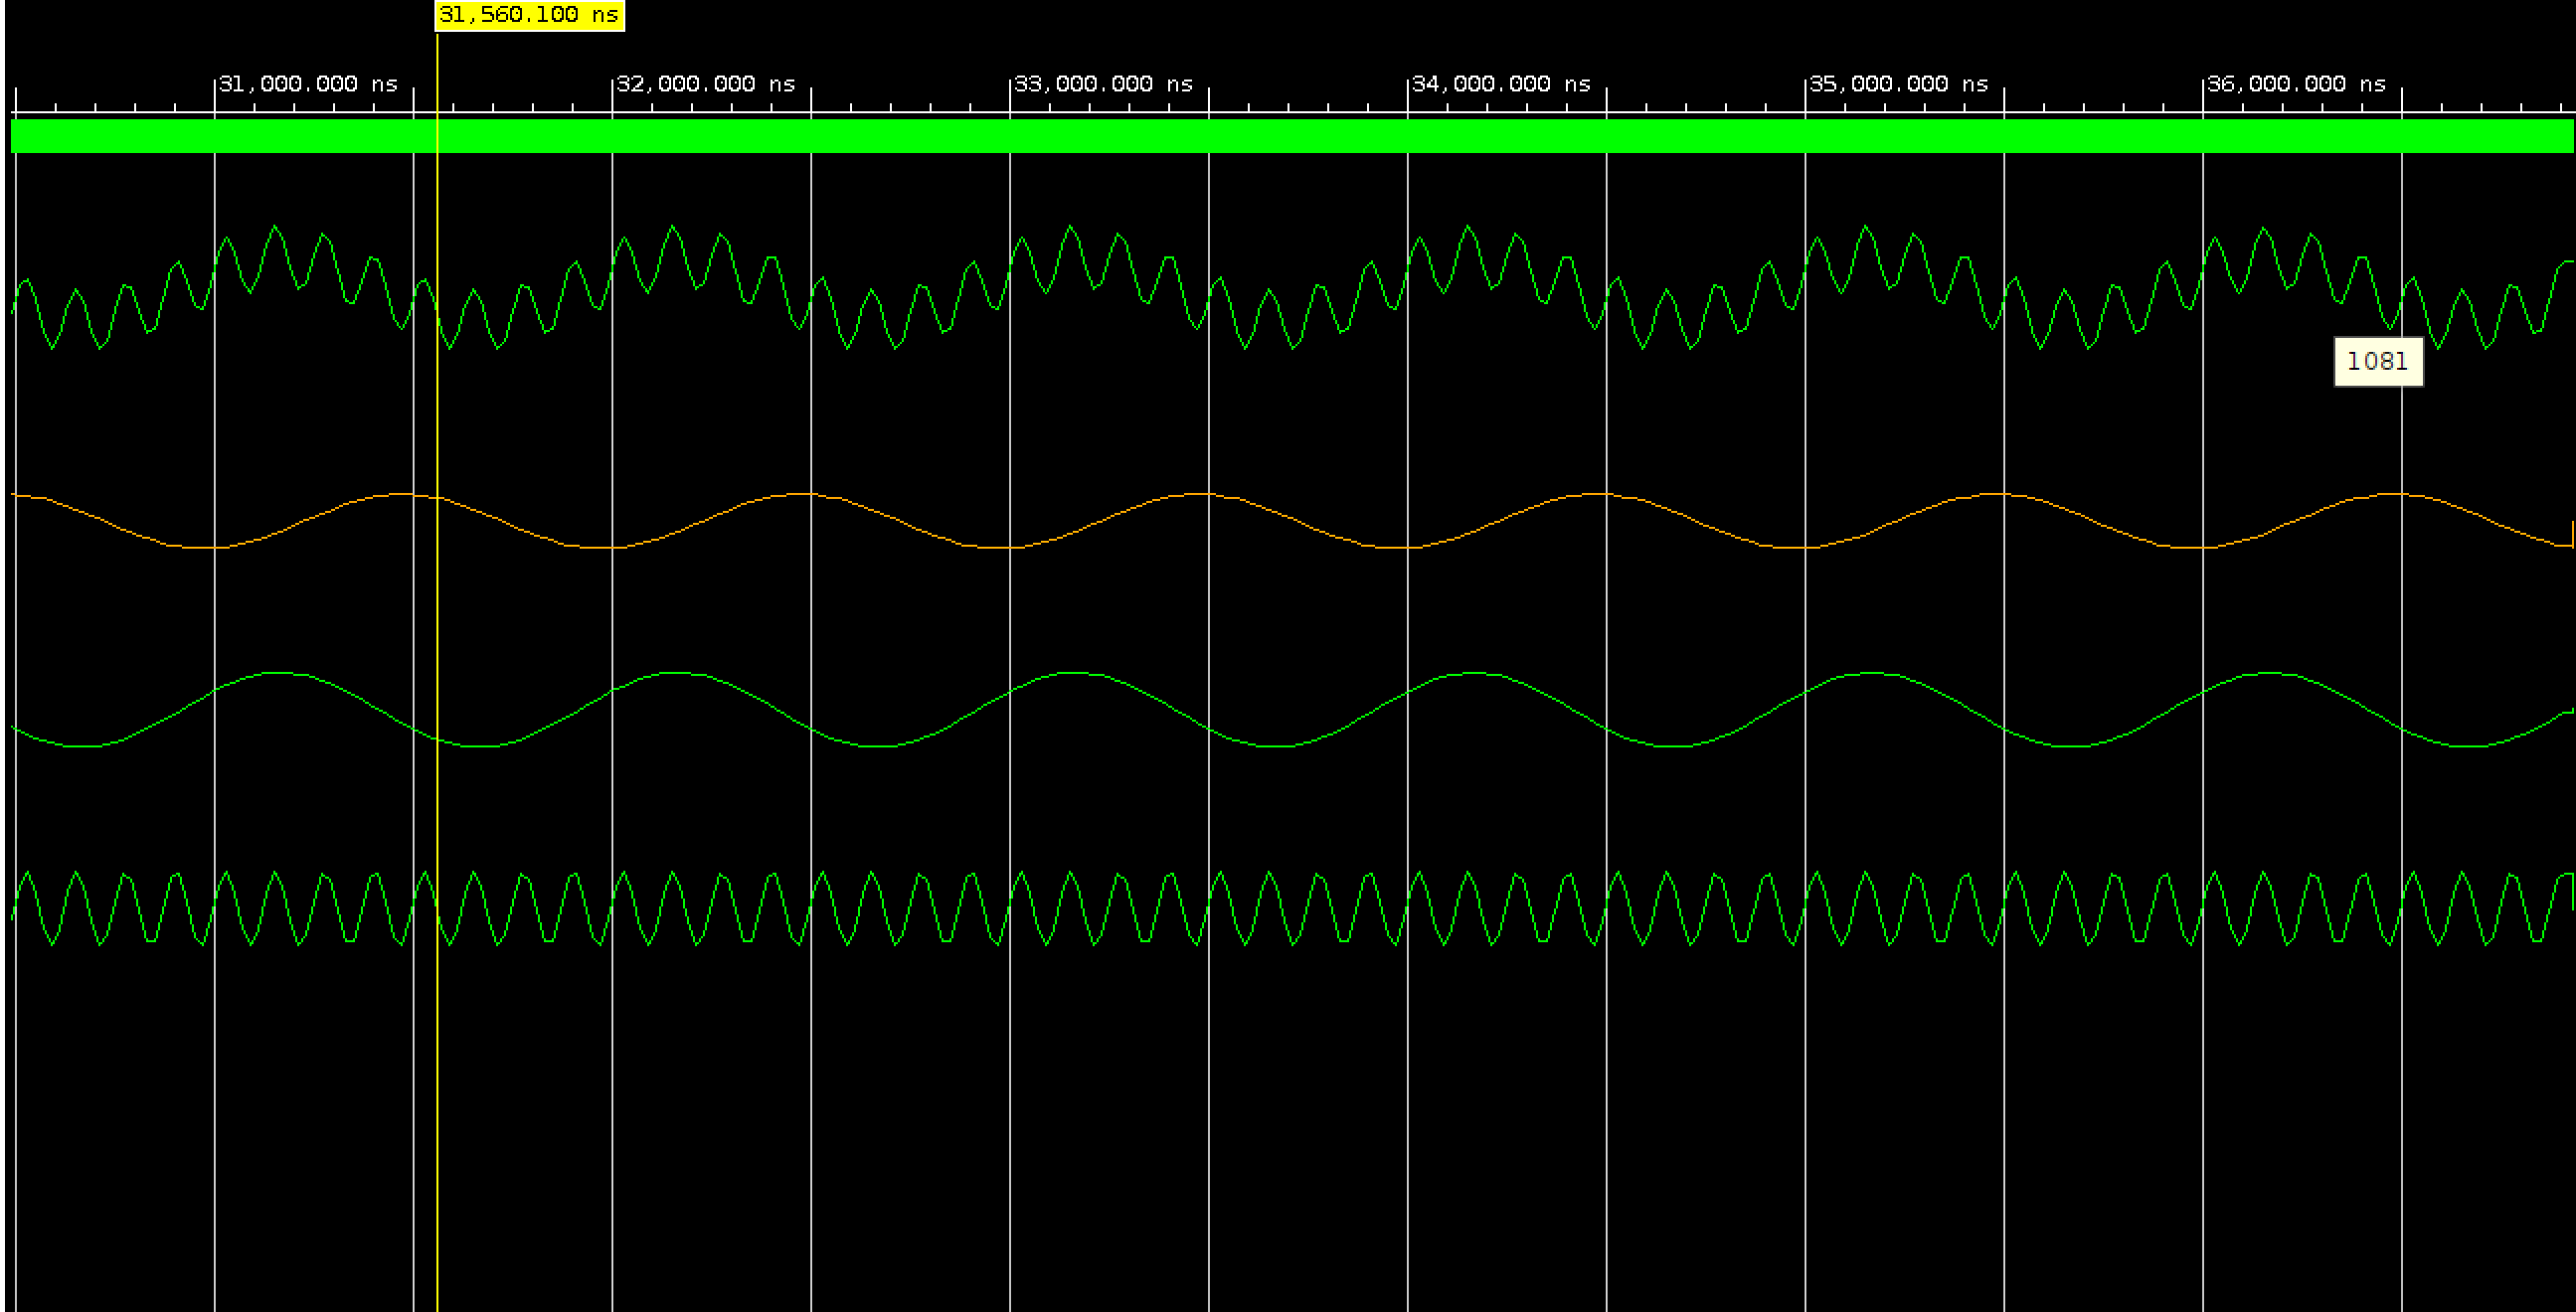
\includegraphics[width=0.75\textwidth]{figure/exp5/waveform.png}
  \caption{FIR滤波器滤波结果}
  \label{fig:exp5:result}
\end{figure}

为了进一步验证该模块的可靠性,将设计部署到FPGA上。在FIR模块之上,复用上一章的顶层模块,并选择滤波前和滤波后的两个信号。由于DAC的输出位宽为14,故对于不满14位的输入数据,按照二进制补码规则向上补齐符号位至14位。\footnote{在模拟域下,相当于幅度缩小16倍,但相对幅度是不变的。}而对大于14位的信号,则选择最高14位(含符号位)截断,舍弃低位。代码如下。

\begin{lstlisting}[language=verilog,caption={顶层模块}]
`timescale 1ns / 1ps
module TOP (
    // DAC  PINS
    output signed [13:0] LS_DAC2_DB,   // DA 数据2
    output               LS_DAC2_CLK,  // DA 时钟2 (125MHz 以下)
    output               LS_DAC2_WRT,  // DA 输出写信号,同时钟信号
    output signed [13:0] LS_DAC1_DB,   // DA 数据1
    output               LS_DAC1_CLK,  // DA 时钟1 (125MHz 以下)
    output               LS_DAC1_WRT,  // DA 输出写信号,同时钟信号

    output LS_DAC_MODE,     

    input PL_CLK_100MHz  // 时钟输入
);

  wire               clk_50M;
  wire               clk_locked;
  wire signed [10:0] sin8M;
  wire signed [10:0] sin1M;
  wire signed [11:0] xin;  //重新定义了两个端口
  wire signed [13:0] xin_new;
  wire signed [25:0] yout;
  clk50m inst_clk50m (
      // Clock out ports
      .clk_out_50m(clk_50M),       // output clk_out_50m
      // Status and control signals
      .locked     (clk_locked),    // output locked
      // Clock in ports
      .clk_in1    (PL_CLK_100MHz)  // input clk_in1
  );

  ila_0 inst_ila (
      .clk(clk_50M),  // input wire clk
      .probe0(xin_new),  // input wire [13:0]  probe0 ,修改为11位 
      .probe1(yout[25:12])  // input wire [13:0]  probe1
  );


  fir_parallel sim (
      .clk(clk_50M),
      .Xin(xin),  // 确保正确连接输入信号
      .Yout(yout)  // 确保正确连接输出信号
  );

  SIN_1M sin_1M (
      .aclk                (clk_50M),  // input wire aclk
      .s_axis_config_tvalid(1'b1),     // input wire s_axis_config_tvalid
      .s_axis_config_tdata (16'H51E),  // input wire [11 : 0] s_axis_config_tdata
      .m_axis_data_tvalid  (),         // output wire m_axis_data_tvalid
      .m_axis_data_tdata   (sin1M)     // output wire [11 : 0] m_axis_data_tdata
  );
  SIN_8M sin_8M (
      .aclk                (clk_50M),   // input wire aclk
      .s_axis_config_tvalid(1'b1),      // input wire s_axis_config_tvalid
      .s_axis_config_tdata (16'H28F5),  // input wire [15 : 0] s_axis_config_tdata
      .m_axis_data_tvalid  (),          // output wire m_axis_data_tvalid
      .m_axis_data_tdata   (sin8M)     // output wire [15 : 0] m_axis_data_tdata
  );

  // 计算输入信号
  assign xin = sin1M + sin8M;
  assign xin_new = {{2{xin[11]}}, xin};  //完成位数的扩展
  // DAC OUTPUT
  assign LS_DAC_MODE = 1'b1;
  assign LS_DAC1_DB = xin_new + 14'h2000;  
  assign LS_DAC1_CLK = !clk_50M;
  assign LS_DAC1_WRT = LS_DAC1_CLK;
  assign LS_DAC2_DB = yout[25:12] + 14'h2000;  //位宽
  assign LS_DAC2_CLK = clk_50M;
  assign LS_DAC2_WRT = LS_DAC2_CLK;

endmodule


\end{lstlisting}

生成TOP模块的比特流,并烧录到FPGA开发板上,可从示波器处看到波形(图~\ref{fig:exp5:Implementation})。
\begin{figure}[htbp]
  \centering
  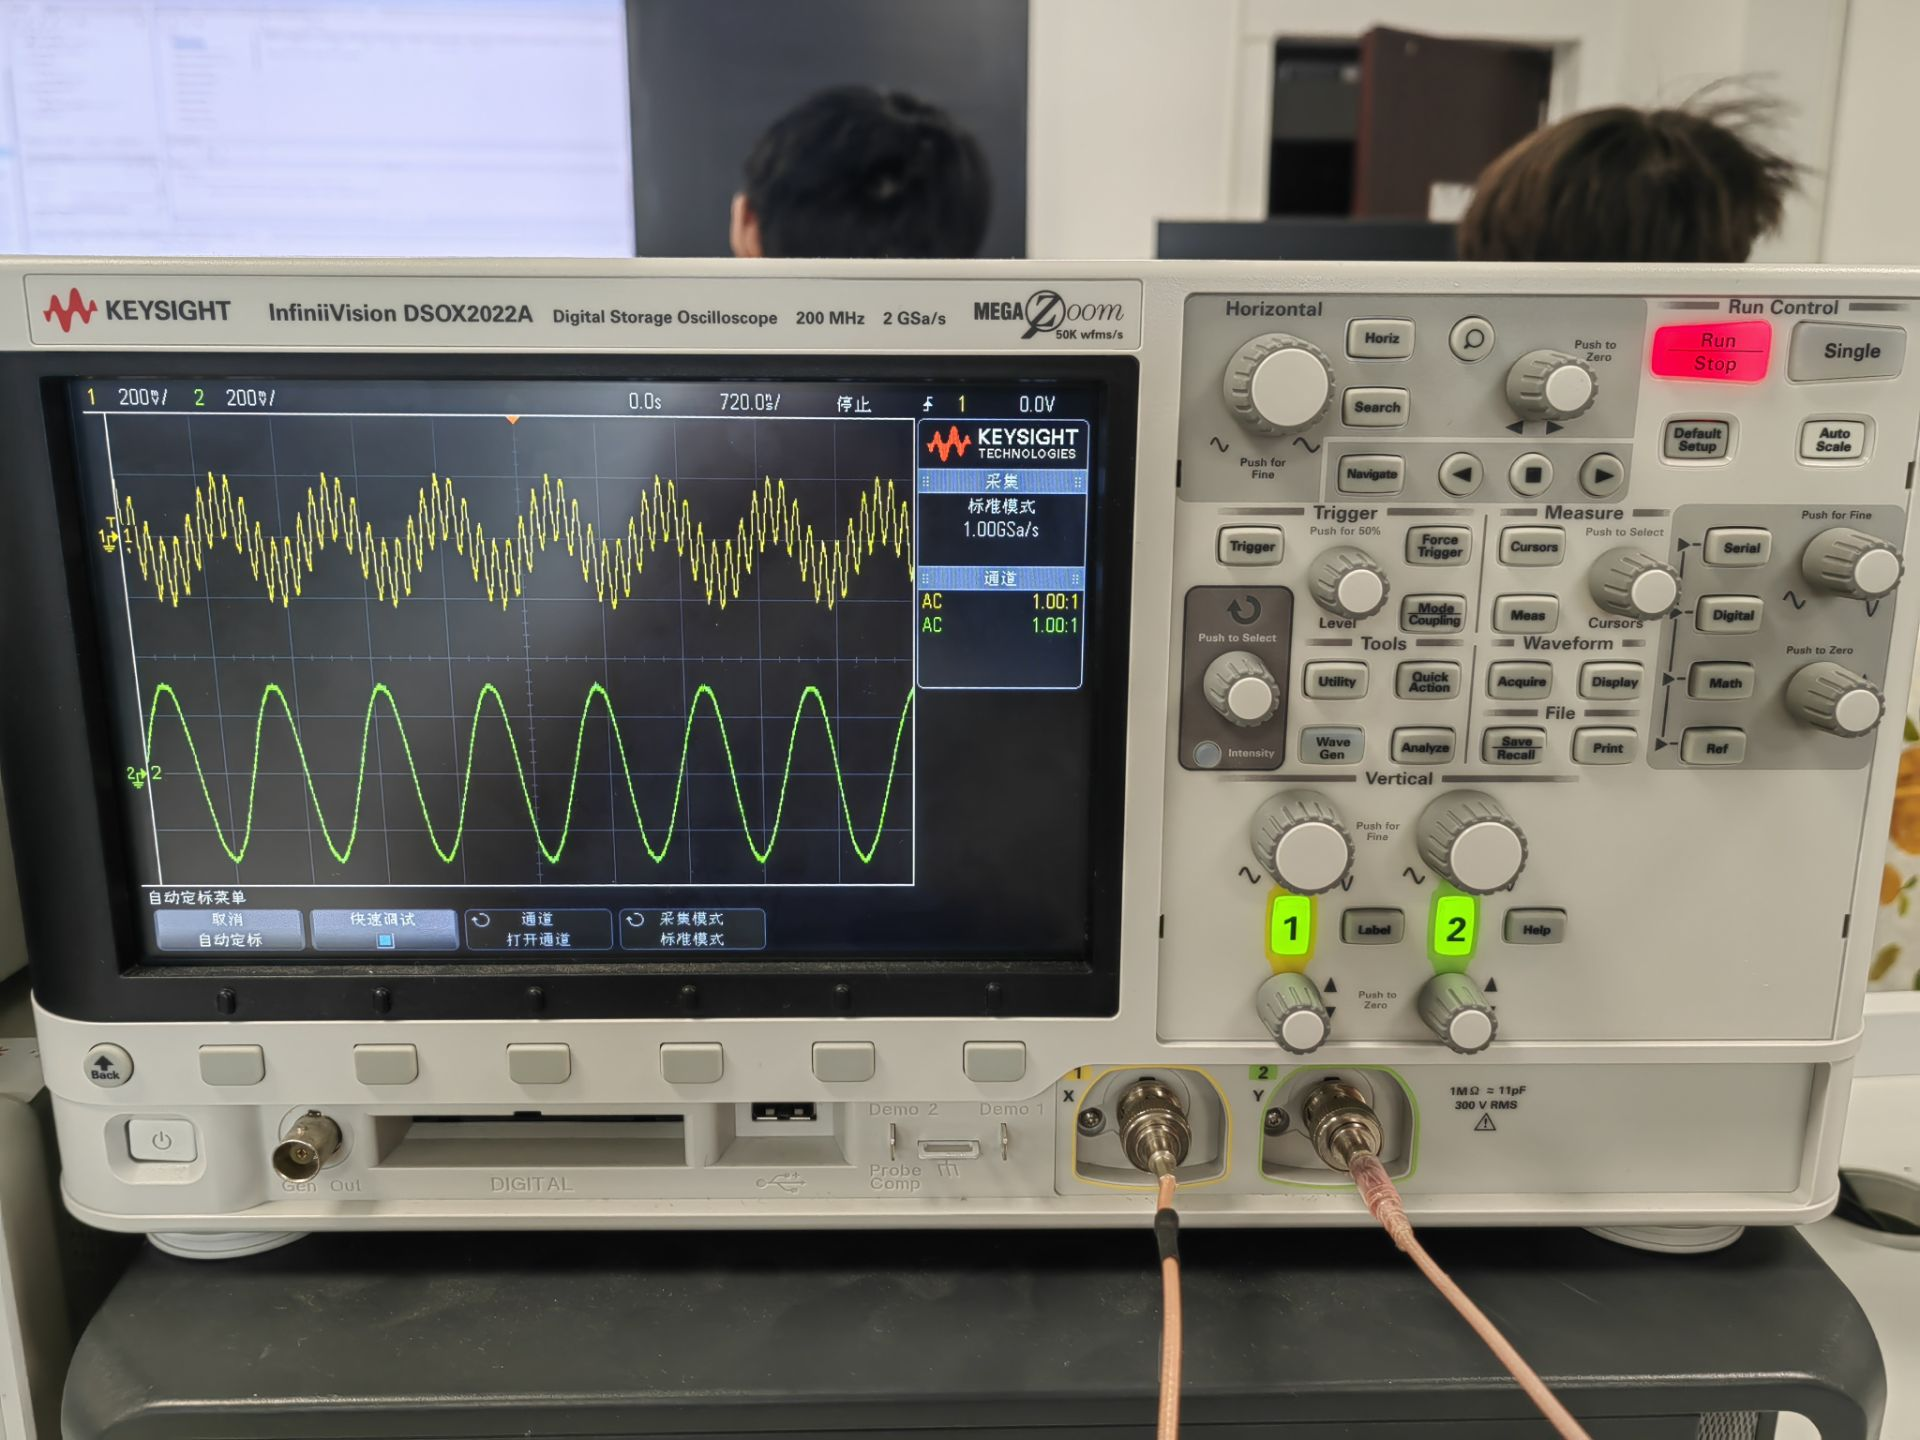
\includegraphics[width = 0.95\textwidth]{figure/exp5/waveform.jpg}
  \caption{滤波前(黄色)与滤波后(绿色)的示波器波形}
  \label{fig:exp5:Implementation}
\end{figure}
\subsection{FPGA资源消耗分析}
首先将该并行滤波器\textbf{设置为顶层模块},并\textbf{禁用}TOP模块。然后通过命令行或\texttt{Add Timing Constraints}绑定时钟管脚\texttt{clk}至50MHz时钟。此时Vivado便可以不通过实际开发板完成资源消耗分析。

完成Implementation后,打开Report Utilization便可看到该模块的资源消耗情况如图~\ref{fig:parrllel:util}。
\begin{figure}[htbp]
  \centering
  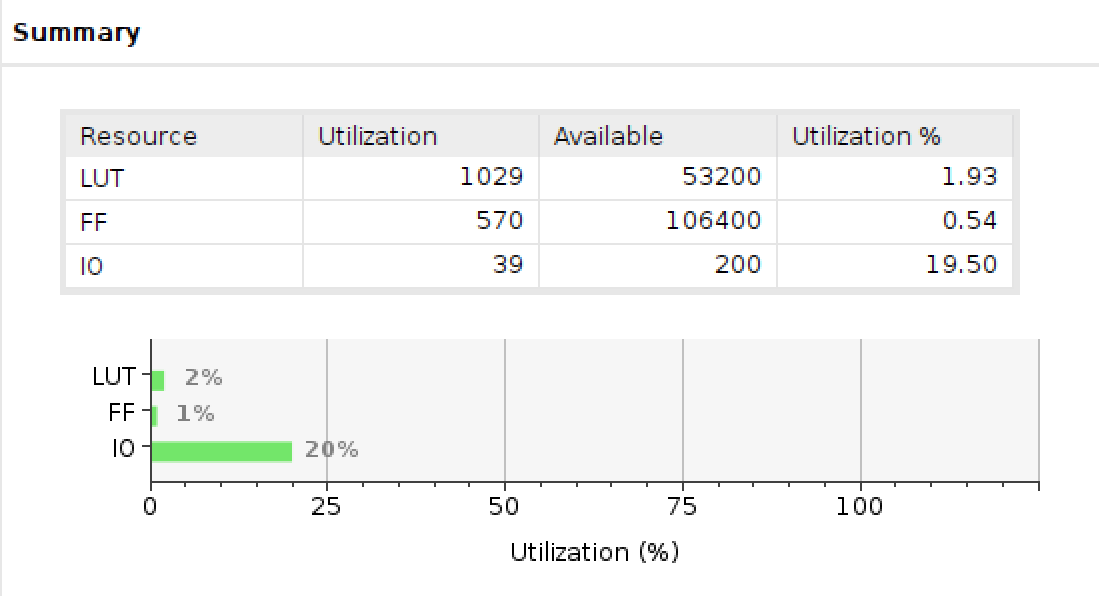
\includegraphics[width=0.55\textwidth]{figure/exp5/util_summary.png}
  \caption{全并行FIR滤波器资源消耗分析}
  \label{fig:parrllel:util}
\end{figure}

该设计的 LUT 和 FF 的资源消耗都很低,但IO资源的消耗较高(19.5\%),这是因为输入输出的位宽较大,属于刚性需求。并且可以看出,在Implementation的过程中,布线器对资源进行了优化。总消耗资源并不等于每个子模块的资源消耗之和。

\subsection{时序检查报告}

图~\ref{fig:exp5:timing}~展示了FPGA设计的时序总结,包括Setup、Hold和Pulse Width三个方面的时序检查结果。

\begin{figure}[htbp]
  \centering
  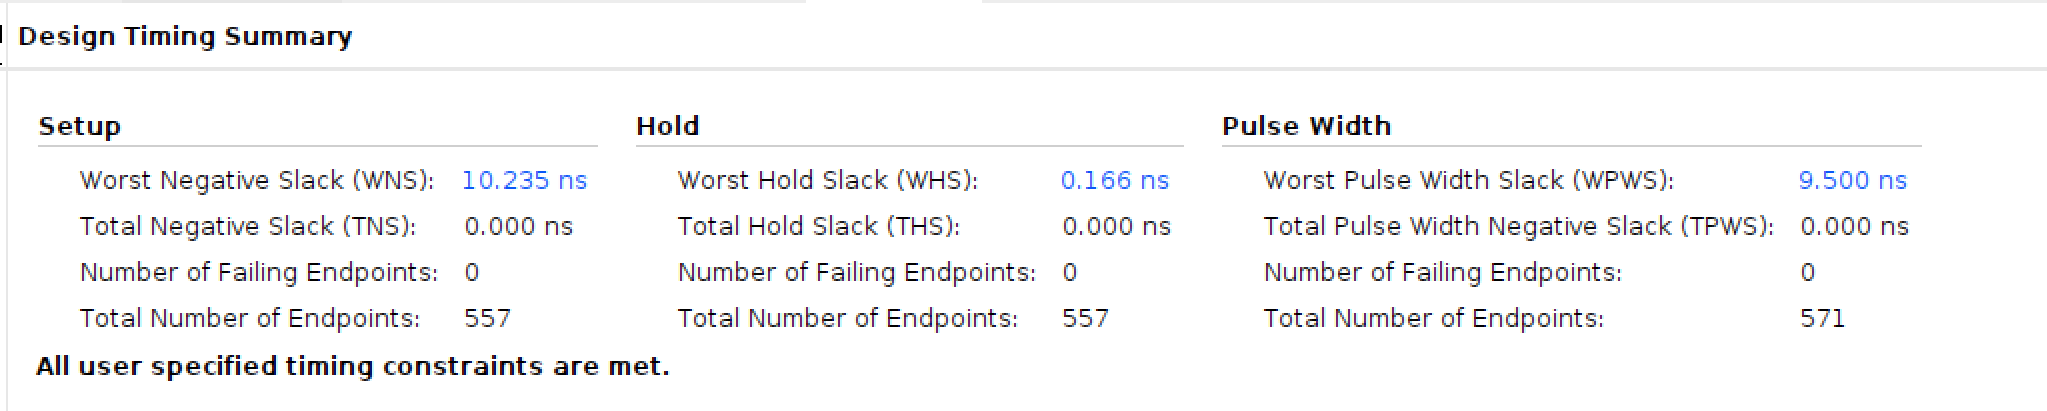
\includegraphics[width=0.75\textwidth]{figure/exp5/timing_summary.png}
  \caption{模块时序检查报告}
  \label{fig:exp5:timing}
\end{figure}


\textbf{Setup:}  
\begin{itemize}
  \item Worst Negative Slack (WNS): 10.235 ns。表示最差的负时序余量,值为10.235纳秒,说明在时序上存在一定的余量,设计没有违反时序约束。  
\item Total Negative Slack (TNS): 0.00 ns。表示总的负时序余量为零,说明所有时序约束都被满足。  
\item Number of Failing Endpoints: 0。表示没有时序失败的端点,所有的时序约束都符合要求。  
\item Total Number of Endpoints: 557。表示在设计中,共有557个时序端点。
\end{itemize}


\textbf{Hold:}  
\begin{itemize}
\item Worst Hold Slack (WHS): 0.166 ns。表示最差的保持时序余量,值为0.166纳秒,表明该设计在保持时序方面没有违反约束。  
\item Total Hold Slack (THS): 0.00 ns。表示总的保持时序余量为零,表明所有保持时序约束都被满足。  
\item Number of Failing Endpoints: 0。表示没有违反保持时序约束的端点。  
\item Total Number of Endpoints: 557。表示共有557个端点。
\end{itemize}

\textbf{Pulse Width:}  
\begin{itemize}
  \item Worst Pulse Width Slack (WPWS): 9.500 ns。表示最差的脉冲宽度时序余量,值为9.500纳秒,说明设计在脉冲宽度方面有足够的时序余量。  
  \item Total Pulse Width Negative Slack (TPWS): 0.00 ns。表示总的脉冲宽度负时序余量为零,表明所有脉冲宽度时序约束都得到满足。  
  \item Number of Failing Endpoints: 0。表示没有违反脉冲宽度时序约束的端点。  
\item Total Number of Endpoints: 571。表示共有571个端点。
\end{itemize}


\textbf{总结:}  
所有用户指定的时序约束都已满足,设计没有违反时序约束,时序余量充足,表明该设计的时序性能良好,符合要求。

\section{思考与讨论}
\subsection{提高该滤波器工作频率的方法}

由于全并行、全展开结构下,大部分逻辑均能在一个时钟周期内完成,因此耗时较久的即为乘法器模块。为了提升乘法器的效率,可以使用以下两种办法:
\begin{enumerate}
  \item 使用DSP资源中的乘法单元代替LUT。
  \item 增加乘法器的并行度。
\end{enumerate}